


Uma abordagem inicial para modelar sistemas físicos consiste em empregar as leis fundamentais da física. Além disso, em situações mais complexas, é viável decompor o sistema em subsistemas menores e, em seguida, desenvolver modelos para cada um deles. Por fim, é possível conectar esses modelos, de forma a obter uma representação aproximada do sistema real. Dessa maneira, podemos obter uma compreensão mais aprofundada e abrangente da dinâmica do sistema em questão. A Figura \ref{fig4:image_01} mostra um diagrama da representação do Aeropêndulo como um conjunto de subsistemas.


\begin{figure}[!h]
	\centering
	\caption{Subsistemas do  Aeropêndulo.}
            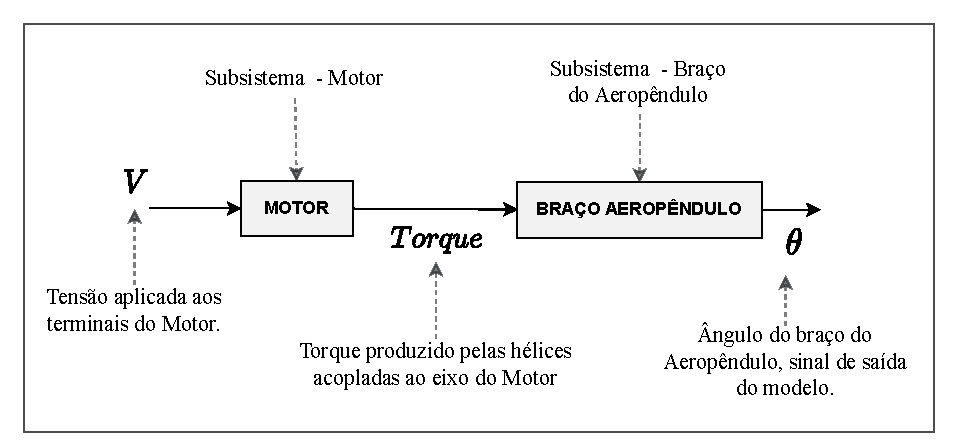
\includegraphics[width=1\textwidth]{Capitulos/4_desenvolvimento/4_figuras/subsistemas_aeropendulo.pdf}
	\caption*{Fonte: elaborado pelo autor (2023).}
        \label{fig4:image_01}
\end{figure}


\subsection{Modelo Matemático do Motor CC Série}
\label{modelagem_motorccserie}

Os motores CC série tem como principal característica possuir o enrolamento de campo em série com o enrolamento de armadora, essa configuração resulta em um motor com torque de partida alto, porém, o torque reduz a medida que a velocidade aumenta devido ao aumento da Força Eletromotriz FEM. Por conta desse aumento de FEM os motores CC Séries tem uma regulação de velocidade ruim, quando se aumenta a carga no eixo do motor a velocidade é reduzida que por sua vez reduz a FEM e então o torque aumenta para conseguir atuar na carga.


\begin{citacao}
    No motor série, o aumento de carga é acompanhado por elevações da corrente,
    da FMM de armadura e do fluxo de campo do estator (desde que o ferro não esteja
    completamente saturado). Como o fluxo aumenta com a carga, a velocidade deve cair
    para se manter o equilíbrio entre a tensão aplicada e a força contraeletromotriz. Além
    disso, o aumento na corrente de armadura, causado pelo aumento de conjugado, é
    menor do que no motor em derivação devido ao aumento de fluxo. O motor série
    é, portanto, um motor de velocidade variável, \citeonline[p.~410]{umans2014}.
\end{citacao}


No entanto, mesmo motores cc série com dimensões reduzidas geram torques altos com baixo consumo de corrente. Visando melhorar seu desempenho, é possível projetar controladores de malha fechada capazes de tornar esses motores mais eficientes na regulação de velocidade.

\cite{jesus} foi usando como base para realizar a modelagem o motor CC série, A Figura \ref{fig4:image_02} mostra um diagrama da configuração do motor CC Série, no qual o enrolamento de campo está conectado em série com o enrolamento de armadura, dessa forma, a  corrente de campo é igual a corrente de armadura $ i = i_f = i_a$.


\begin{figure}[!h]
	\centering
	\caption{Motor CC Série.}
	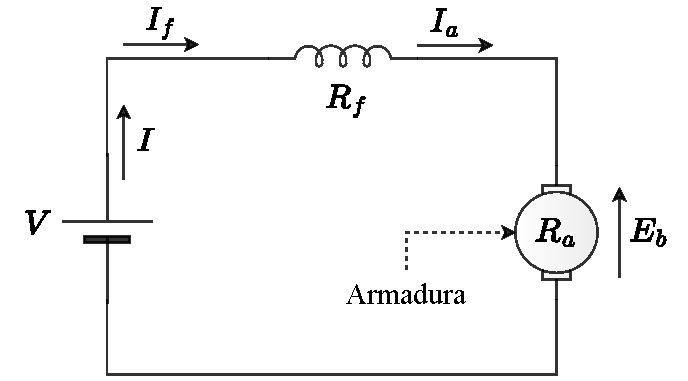
\includegraphics[width=0.7\textwidth]{Capitulos/4_desenvolvimento/4_figuras/esquema_motor_cc.pdf}
	\caption*{Fonte:  elaborado pelo autor (2023).}
	\label{fig4:image_02}
\end{figure}

Na Figura \ref{fig4:image_03}, mostra o diagrama eletromecânico do motor, nele pode-se observar que os componentes elétricos estão todos em série, no qual o enrolamento de campo possui uma parte resistiva e outra indutiva, assim como o enrolamento de armadura, já a parte mecânica possui uma velocidade angular dada por $\dot{\omega}$, torque eletromagnético do motor dado por $T_e$ e torque da Carga $T_c$.


\begin{figure}[!h]
	\centering
	\caption{Diagrama Elétrico/Mecânico Motor CC Série.}
	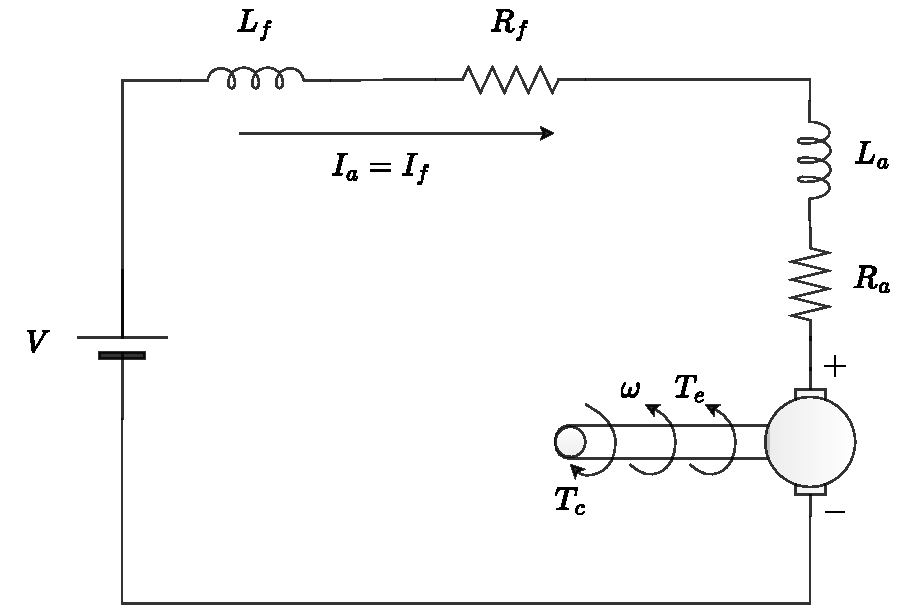
\includegraphics[width=0.6\textwidth]{Capitulos/4_desenvolvimento/4_figuras/diagrama_motor_cc.pdf}
	\caption*{Fonte: elaborado pelo autor (2023).}
	\label{fig4:image_03}
\end{figure}


%%%%%%%%%%%%%%%%%%%%%%%%%%%%%%%%%%%%%%%%%%%%%%%%%%%%%%%%%%%%%%%%%%%%%%%%%%%%%%%%%%%%%%%%%%%%%%%%%%%%%%%%%%%%%%%%%%%%%%%%%%%%%%%%%%%%%%%%%
%%%%%%%%%%%%%%%%%%%%%%%%%%%%%%%%%%%%%%%%%%%%% Modelagem da Parte Mecânica do Motor CC Série %%%%%%%%%%%%%%%%%%%%%%%%%%%%%%%%%%%%%%%%%%%%%
%%%%%%%%%%%%%%%%%%%%%%%%%%%%%%%%%%%%%%%%%%%%%%%%%%%%%%%%%%%%%%%%%%%%%%%%%%%%%%%%%%%%%%%%%%%%%%%%%%%%%%%%%%%%%%%%%%%%%%%%%%%%%%%%%%%%%%%%%

\subsubsection{Modelagem da Parte Mecânica do Motor CC Série}

Primeiramente a parte mecânica do motor será modelada, um motor cc série é composto por uma parte rotativa "armadura", de modo que, essa parte, gera um momento de inércia $J_m$ no eixo do motor e um fator de amortecimento viscoso $b$, além disso, o eixo possui uma velocidade angular $\dot{\omega}$.

Assim, a equação \ref{eq4:eq1}, obtida a partir de \cite{jesus}, descreve o modelo mecânico do motor CC Série.

\begin{align}
	J_m\ddot{\omega}(t) &= T_e(t) - b\dot{\omega}(t) - T_c(t) \label{eq4:eq1}
\end{align}


Ao expressar o torque $T_e(t)$ em função das outras variáveis, obtém-se a equação \ref{eq4:eq2}.

\begin{align}
	T_e(t) &= J_m\ddot{\omega}(t) + b\dot{\omega}(t) + T_c(t) \label{eq4:eq2}
\end{align}


Onde:
\begin{itemize}
        \setlength{\itemsep}{-2pt}
	\item $T_e$: Torque Eletromagnético produzido pelo Motor;
	\item $J_m$: Momento de Inércia do Eixo do Motor;
	\item $\ddot{\omega}$: Aceleração Angular do Eixo do Motor;
	\item $\dot{\omega}$: Velocidade Angular do Eixo do Motor;
	\item $b$: Fator de Amortecimento Viscoso;
	\item $T_c$: Torque de Carga.
\end{itemize}

Tanto a Força Eletromotriz $E_A(t)$ quanto o Torque Eletromagnético $T_e(t)$ dependem do fluxo magnético do entreferro $\Phi$, com isso, tem-se as equações \ref{eq4:eq3} e \ref{eq4:eq4}.

\begin{align}
	E_a(t) &= \dot{\omega}(t) \Phi{(i)} \label{eq4:eq3}\\
	T_e(t) &= i(t) \Phi{(i)}			\label{eq4:eq4}
\end{align}

O Fluxo magnético depende da corrente $i(t)$, assim, as equações \ref{eq4:eq1} e \ref{eq4:eq2} são não-lineares. Além disso, pode-se aproximar o fluxo $\Phi$ por uma relação linear, $K_0$, ao desprezar a saturação magnética.

\begin{align}
	\Phi(i) &= K_0 i(t) \label{eq4:eq5}
\end{align}

A constante $K_0$ é a indutância mútua entre a armadura e o enrolamento de campo. Agora pode-se encontrar o modelo não-linear da parte mecânica do Motor CC Série, substituindo \ref{eq4:eq5} em \ref{eq4:eq4}, obtém-se a expressão \ref{eq4:eq7}:

\begin{align}
	T_e(t) &= i(t) K_0 i(t) \label{eq4:eq6}\\
	T_e(t) &= K_0 i^2(t) 	\label{eq4:eq7}
\end{align}

Substituindo \ref{eq4:eq7} em \ref{eq4:eq2}, é possível encontrar o modelo da parte mecânica do motor CC série, assim, tem-se a expressão  \ref{eq4:eq8}.


\begin{align}
	K_0 i^2(t) &= J_m\ddot{\omega}(t) + b\dot{\omega}(t) + T_c(t) \label{eq4:eq8}
\end{align}


%%%%%%%%%%%%%%%%%%%%%%%%%%%%%%%%%%%%%%%%%%%%%%%%%%%%%%%%%%%%%%%%%%%%%%%%%%%%%%%%%%%%%%%%%%%%%%%%%%%%%%%%%%%%%%%%%%%%%%%%%%%%%%%%%%%%%%%%%
%%%%%%%%%%%%%%%%%%%%%%%%%%%%%%%%%%%%%%%%%%%%% Modelagem da Parte Elétrica do Motor CC Série %%%%%%%%%%%%%%%%%%%%%%%%%%%%%%%%%%%%%%%%%%%%%
%%%%%%%%%%%%%%%%%%%%%%%%%%%%%%%%%%%%%%%%%%%%%%%%%%%%%%%%%%%%%%%%%%%%%%%%%%%%%%%%%%%%%%%%%%%%%%%%%%%%%%%%%%%%%%%%%%%%%%%%%%%%%%%%%%%%%%%%%

\subsubsection{Modelagem da Parte Elétrica do Motor CC Série}

Para a parte elétrica, utilizou-se a lei de Kirchhoff das tensões para modelar o sistema. assim como a parte mecânica, o modelo da parte elétrica foi baseado de \cite{jesus}, o motor em questão é um motor de corrente contínua CC série, Dessa forma, $i_a = i_f$, portanto, obtém-se a expressão \ref{eq4:eq9}.


\begin{align}
	V(t) &= (R_a + R_f)i(t)+ (L_a + L_f)\dfrac{d}{dt}i(t) + E_a \label{eq4:eq9}
\end{align}

Onde:

\begin{itemize}
        \setlength{\itemsep}{-2pt}
	\item $V$: Tensão da Fonte;
	\item $R_a$: Resistência da Armadura;
	\item $R_f$: Resistência de Campo;
	\item $i_a$: Corrente da Armadura;
	\item $i_f$: Corrente de Campo;
	\item $E_A$: Tensão Contro Eletromotriz Gerada pela Armadura;
	\item $L_a$: Impedância da Armadura;
	\item $L_f$: Impedância de Campo.
\end{itemize}

Como os componentes elétricos então em série, pode-se obter uma resistência total assim como uma indutância:

\begin{align}
	R &= R_a + R_f          \label{eq4:eq10}\\        
	L &= L_a + L_f          \label{eq4:eq11}
\end{align}

\begin{align}
	V(t) &= Ri(t)+ L\dfrac{d}{dt}i(t) + E_a \label{eq4:eq12}
\end{align}

Substituindo \ref{eq4:eq5} em \ref{eq4:eq3}, obtém-se a equação \ref{eq4:eq13}.

\begin{align}
	E_a(t) &= \dot{\omega}(t)K_0 i(t) \label{eq4:eq13}
\end{align}

Por fim, pode-se encontrar a equação que descreve a parte elétrica do sistema ao substituir \ref{eq4:eq13} em \ref{eq4:eq12}, assim, obtendo a equação \ref{eq4:eq14}.

\begin{align}
	V(t) &= Ri(t)+ L\frac{d}{dt}i(t) + \dot{\omega}(t)K_0 i(t) \label{eq4:eq14}
\end{align}

Dessa forma, as equações que modelam um Motor CC série são expressas por \ref{eq4:eq15} e \ref{eq4:eq16}, em que \ref{eq4:eq15} esta relacionada a parte mecânica e \ref{eq4:eq16} a parte elétrica.

\begin{align}
	K_0 i^2(t) &= J_m\ddot{\omega}(t) + b\dot{\omega}(t) + T_c(t) \label{eq4:eq15}\\
	V(t) &= Ri(t)+ L\dfrac{d}{dt}i(t) + \dot{\omega}(t)K_0 i(t) \label{eq4:eq16}
\end{align}

\vspace{1cm}

\subsubsection{Linearização do modelo do Motor CC Série}

Para projetos de controle lineares é preciso linearizar o modelo encontrado, para isso, vamos reorganizar as equações \ref{eq4:eq15} e \ref{eq4:eq16}, assim obtêm-se as equações \ref{eq4:eq17} e \ref{eq4:eq18}:

\begin{align}
    \ddot{\omega}(t) &= \dfrac{K_0}{J_m} i^2(t) - \frac{b}{J_m}\dot{\omega}(t) - \dfrac{1}{J_m}T_c(t) \label{eq4:eq17}\\
    \dfrac{d}{dt}i(t) &= \dfrac{R}{L}i(t)- \dfrac{K_0}{L}\dot{\omega}(t)i(t) +\dfrac{1}{L}V(t) \label{eq4:eq18}
\end{align}

reescrevendo as equações de estados na forma matricial,

\begin{align}
    x_1 = \dot{\omega}  \label{eq4:eq19}\\
    x_2 = i   \label{eq4:eq20}
\end{align}


Coeficientes da equação de estado \ref{eq4:eq17}.

\begin{align}
    a_1 = \dfrac{K_0}{J_m}; \quad a_2 = \dfrac{b}{J_m}; \quad a_3 = \dfrac{1}{J_m}  \label{eq4:eq21}
\end{align}

Coeficientes da equação de estado \ref{eq4:eq18}.

\begin{align}
    b_1 = \dfrac{R}{L}; \quad b_2 = \dfrac{K_0}{L}; \quad b_3 = \dfrac{1}{L}  \label{eq4:eq22}
\end{align}

Representação no espaço de estados do motor CC Série não-linear

\begin{align}
    \dot{x}_1 &= a_1x_2^2  - a_2x_1 -a_3T_c   \label{eq4:eq23}\\
    \dot{x}_2 &= -b_1x_2  -b_2x_1x_2 + b_3V    \label{eq4:eq24}
\end{align}



\begin{align}
\dot{x} = \begin{bmatrix}
    \dot{x}_1\\
    \dot{x}_2
\end{bmatrix} = 
\begin{bmatrix}
    a_1x_2^2 -a_2x_1 -a_3T_c \\
    -b_1x_2 -b_2x_1x_2 + b_3V
\end{bmatrix} = f(x, u)  \label{eq4:eq25}
\end{align}

O ponto de equilíbrio $(x_1^0, x_2^0)$ das equações \ref{eq4:eq23} e \ref{eq4:eq24} é encontrado zerando as derivadas, como mostrado em \ref{eq4:eq26} e \ref{eq4:eq27}.


\begin{align}
     x_2^0 &= \sqrt{\frac{a_2x_1^0 + a_3T_c}{a_1}} \label{eq4:eq26}\\
     V &= \frac{x_2^0(b_1+b_2x_1^0)}{b_3} \label{eq4:eq27}
\end{align}


A linearização de  \ref{eq4:eq23} e \ref{eq4:eq24} em torno do ponto de equilíbrio é obtida encontrando o jacobiano das mesmas, assim se obtêm as matrizes $A$ e $B$.

\begin{align}
     \dot{x} &= Ax + Bu    \label{eq4:eq28}\\
     y &= Cx               \label{eq4:eq29}
\end{align}

Em que, 

\begin{align}
     A &= \left. \dfrac{\partial f(x,y)}{\partial x}\right|_{x_1^0, x_2^0} = \begin{bmatrix}
    -a_2       &   2a_1x_2^0\\
    -b_2x_2^0  & -(b_1+b_2x_1^0)
\end{bmatrix}    \label{eq4:eq30}\\
B &= \left. \dfrac{\partial f(x,y)}{\partial u}\right|_{x_1^0, x_2^0} = \begin{bmatrix}
    -a_3       &   0\\
    0  & b_3
\end{bmatrix}    \label{eq4:eq31}\\
C &= [1, 0]      \label{eq4:eq32}\\
\end{align}


Onde,

\begin{align}
    u &= \begin{bmatrix}
        T_c\\
        V
\end{bmatrix}           \label{eq4:eq33}\\
y &= \dot{\omega}(t)    \label{eq4:eq34}
\end{align}


Se o torque de carga for considerado zero, $T_c = 0$, temos as seguintes expressões,

\begin{align}
     x_2^0 = \sqrt{\frac{a_2x_1^0}{a_1}}; \quad
         V = \frac{x_2^0(b_1+b_2x_1^0)}{b_3}; \quad
         B = \begin{bmatrix}
        0\\
        b_3
\end{bmatrix}  \label{eq4:eq35}
\end{align}

Agora é possível encontrar a função de transferência $G(s)$ associada as matrizes de estados $A, B, C$ linearizadas, para isso usa-se a expressão \ref{eq4:eq36}.


\begin{align}
    G(s) &= \frac{\dot{\omega}(s)}{V(s)} = C(sI-A)^{-1}B     \label{eq4:eq36}
\end{align}

Substituindo as matrizes $A$, $B$ e $C$ em \ref{eq4:eq36}, chega-se a expressão \ref{eq4:eq36_1}.

\begin{align}
    G(s) &= \frac{\dot{\omega}(s)}{V(s)} = \begin{bmatrix}
        1 & 0
\end{bmatrix} \cdot \left(s \cdot \begin{bmatrix}
    1  & 0\\
    0  & 1
\end{bmatrix}-\begin{bmatrix}
    -a_2       &   2a_1x_2^0\\
    -b_2x_2^0  & -(b_1+b_2x_1^0)
\end{bmatrix}\right)^{-1} \cdot \begin{bmatrix}
    -a_3       &   0\\
    0  & b_3
\end{bmatrix}     \label{eq4:eq36_1}
\end{align}

Assim, obtém-se a função de transferência linearizada em função dos parâmetros do motor CC Série, como mostra a equação \ref{eq4:eq37}.



\begin{align}
    G(s) &= \frac{\dot{\omega}(s)}{V(s)} = \dfrac{2 K_{0} \sqrt{\dfrac{b x^{0}_{1}}{K_{0}}}}{J_m L s^{2} + 3 K_{0} b x^{0}_{1} + R b + s \left(J_m K_{0} x^{0}_{1} + J_m R + L b\right)}     \label{eq4:eq37}
\end{align}

\vspace{1cm}

\subsection{ Modelo Matemático Braço do Aeropêndulo}
\label{modelagem_braco_aeropendulo}

Os sistemas mecânicos têm como uma de suas característica os graus liberdade, da sigla em inglês 6DoF - (Six degrees of freedom) que em português que dizer (Seis graus de liberdade), com esses seis graus de liberdade é possível mover a planta em todas as direções e ângulos, o aeropêndulo tem um grau de liberdade, sendo o ângulo $\theta$, assim o sistema tem apenas uma variável a ser controlada a partir do empuxo gerado pelas hélices, que por sua vez depende da velocidade angular do eixo do motor CC Série acoplado ao braço do aeropêndulo. dessa forma, podemos analisar o sistema a partir da entrada e da saída, sendo a entrada a tensão no motor e a saída o ângulo $\theta$ do braço do aeropêndulo.

como discutido antes, pode-se dividir o sistema em dois subsistemas, o motor CC Série e o braço do aeropêndulo. para o motor CC Série, já foi realizado a modelagem na sessão \ref{modelagem_motorccserie}, para essa sessão será realizada a modelagem do braço do aeropêndulo, \cite{amin} foi usando como base para se obter a equação que modela a dinâmica do braço.

\begin{figure}[!h]
	\centering
	\caption{Diagrama esquemático do Aeropêndulo.}
	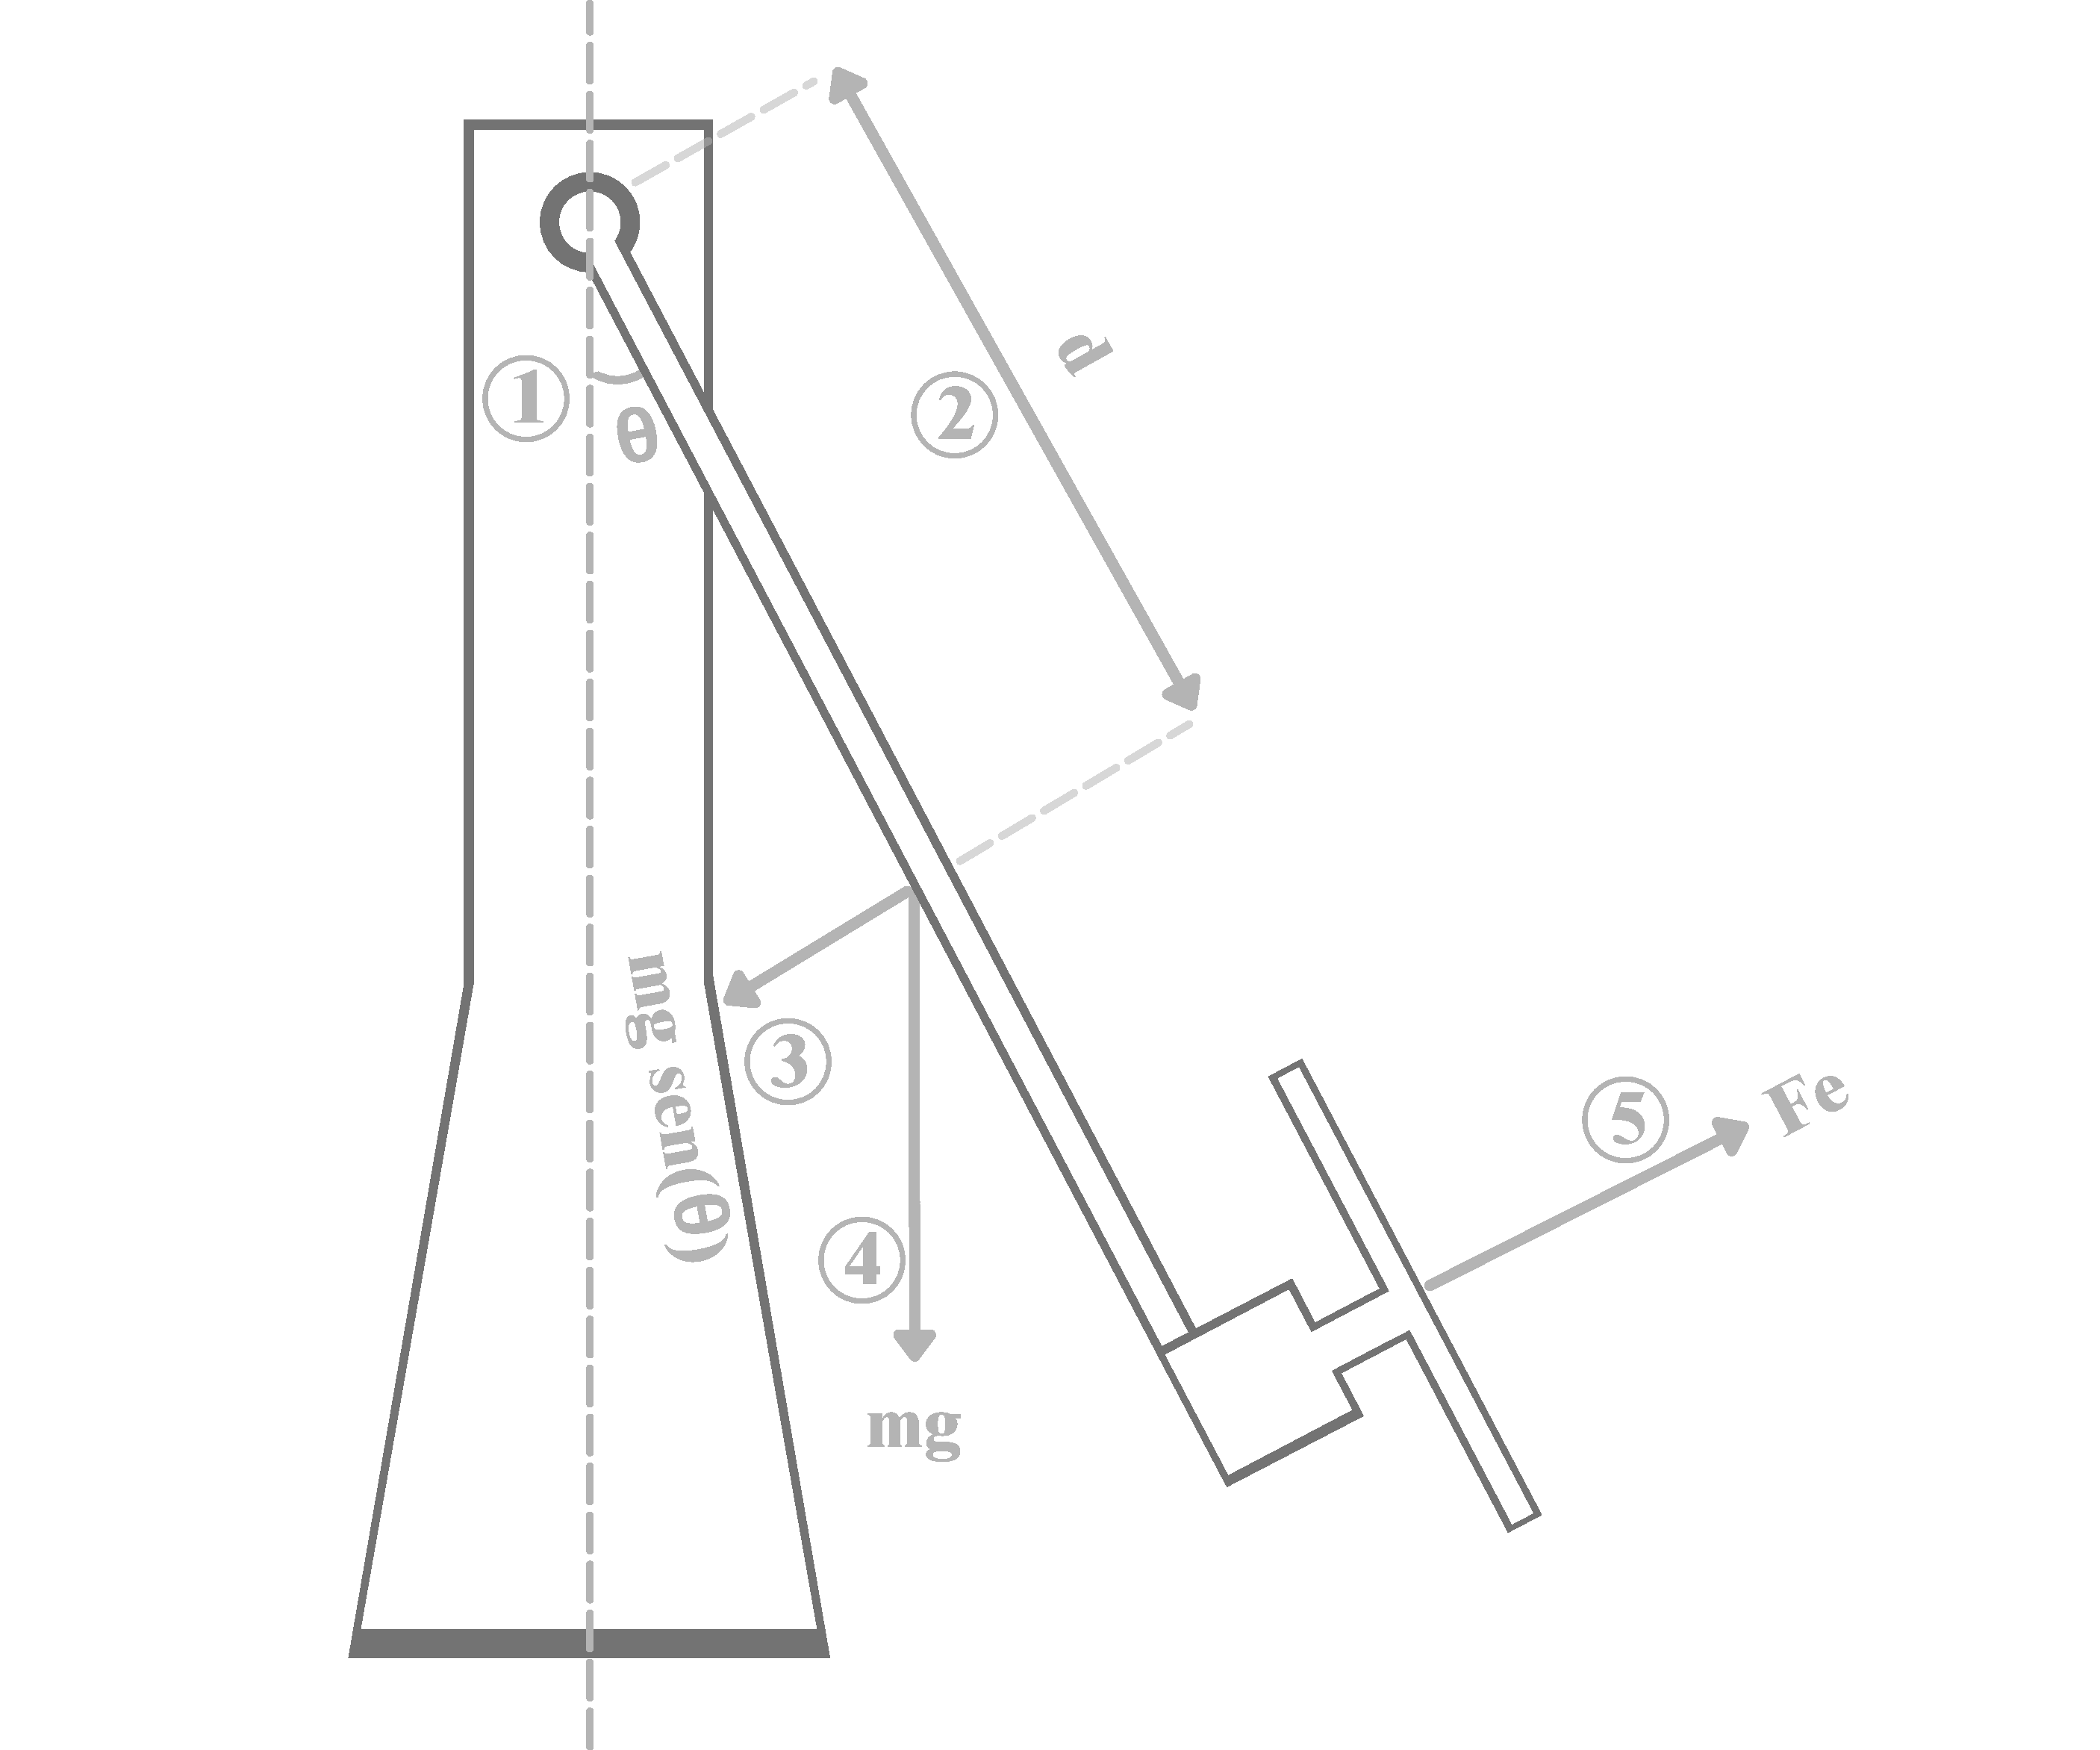
\includegraphics[width=0.65\textwidth]{Capitulos/4_desenvolvimento/4_figuras/desenho_aeropendulo.pdf}
	\caption*{Fonte: elaborado pelo autor (2023).}
        \label{fig4:image_04}
\end{figure}


O modelo matemático do braço do aeropêndulo é derivado a partir das leis de Newton e do momento angular, como mostra \cite{amin}. assim, se obtém a equação \ref{eq4:eq38}.

\begin{align}
    F_e &= J_b\ddot{\theta} + c\dot{\theta} +mgd\sin{\theta}  \label{eq4:eq38}
\end{align}

Onde:

\begin{itemize}
        \setlength{\itemsep}{-2pt}
	\item  $F_e$: Empuxo gerado pela hélice
        \item  $J_b$: Momento de inércia do Braço
        \item  $\theta$: posição angular do Aeropêndulo
        \item  $c$: coeficiente de amortecimento viscoso
        \item  $m$: massa do Aeropêndulo
        \item  $d$: a distância entre o centro de massa e o ponto de pivô
\end{itemize}

A entrada do subsistema do braço do aeropêndulo é a força de empuxo proporcionada pela hélice, porém, o modelo do motor CC Série tem como saída a velocidade angular, dessa forma é preciso encontrar uma relação entre a velocidade $\dot{\omega}$ e o empuxo $F_e$, essa relação é não linear como mostra $[xx]$, $F_e = K_m\dot{\omega}^2$, porém é possível aproximar por uma relação linear,  $F_e = K_m\dot{\omega}$. Com isso, pode-se relacionar a velocidade angular $\dot{\omega}$  com o empuxo $F_e$ gerado pela hélice do aeropêndulo.

O modelo encontrado tem uma parcela não linear dada por $\sin{\theta}$, para aplicar técnicas de projeto de controle é preciso obter o modelo linearizado da planta, isso pode ser feito considerando $\sin{\theta} \approx \theta$ para pequenas variações em torno de $\theta$. dessa forma, temos a seguinte linearização:
\begin{align}
    F_e &= J_b\ddot{\theta} + c\dot{\theta} +mgd\theta
    \label{eq4:eq39}
\end{align}

Aplicando a transformada de Laplace para encontrar a função de transferência do subsistema, tem-se:

\begin{align}
    F_e(s) &= s^2J_b\theta(s) + sc\theta(s) +mgd\theta(s) \label{eq4:eq41}\\
    F_e(s) &= (s^2J_b + sc +mgd)\theta(s) \label{eq4:eq42}\\
    \dfrac{\theta(s)}{F_e(s)} &= \frac{1}{s^2J_b + sc +mgd} \label{eq4:eq43}
\end{align}


Agora que foi obtido o modelo do braço do aeropêndulo, pode-se usar a relação linearizada $F_e = K_m\dot{\omega}$ para usar a saída do modelo do motor cc série como entrada do modelo do braço do aeropêndulo, como mostrado na equação \ref{eq4:eq46}.

\begin{align}
    \dfrac{\theta(s)}{K_m\dot{\omega}(s)} &= \dfrac{1}{s^2J_b + sc +mgd} \label{eq4:eq44}\\
    \dfrac{\theta(s)}{\dot{\omega}(s)} &= \dfrac{K_m}{s^2J_b + sc +mgd} \label{eq4:eq45}\\
    H(s) = \dfrac{\theta(s)}{\dot{\omega}(s)} &= \dfrac{\dfrac{K_m}{J_b}}{s^2 + s\dfrac{c}{J_b} +\dfrac{mgd}{J_b}} \label{eq4:eq46}
\end{align}


A equação  \ref{eq4:eq46} é a função de transferência do braço do aeropêndulo.

%\vspace{1cm}
\subsection{Junção dos subsistemas}
\label{junca0_submodelos}

A partir dos modelos encontrados nas subseções \ref{modelagem_motorccserie} e \ref{modelagem_braco_aeropendulo} pode-se obter o modelo completo do sistema unindo os subsistemas como mostra a figura \ref{fig4:image_05}. com isso, é possível modelar o Aeropêndulo tendo como entrada a tensão no motor CC série e como saída o ângulo do braço.

\begin{figure}[!h]
	\centering
	\caption{Diagrama da junção dos subsistemas do  Aeropêndulo.}
            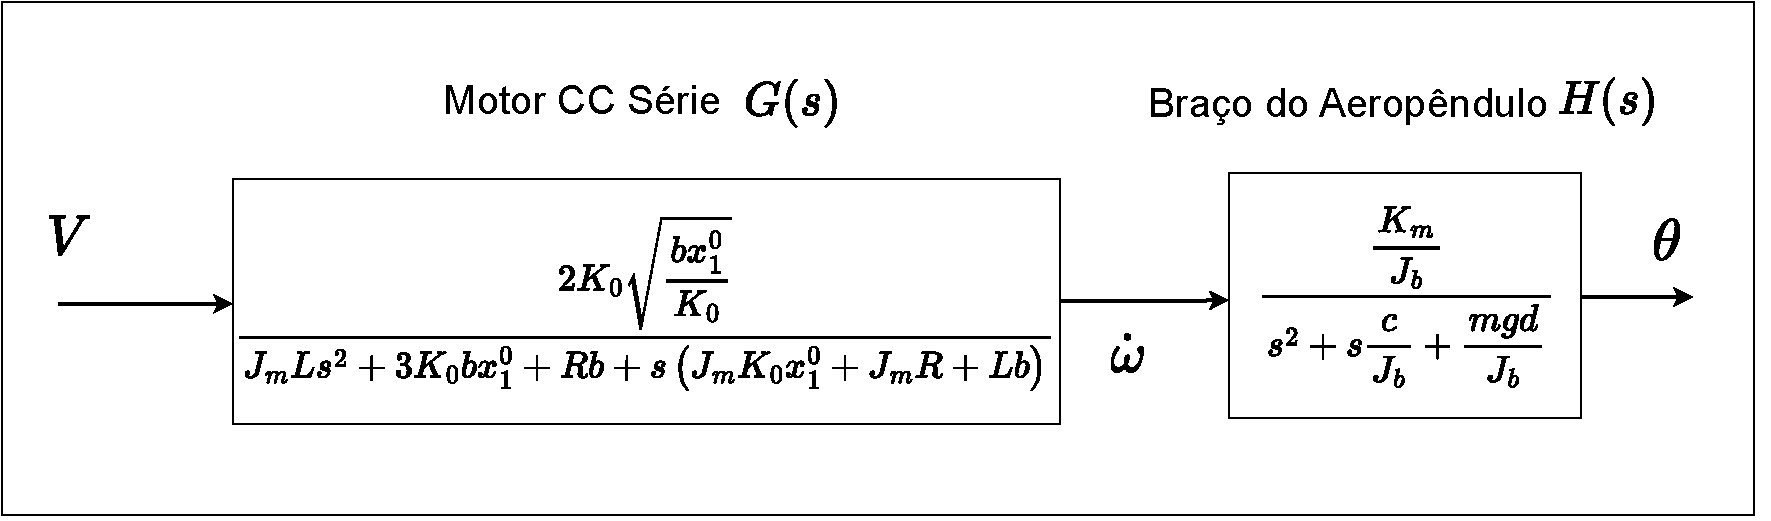
\includegraphics[width=1\textwidth, page=1]{Capitulos/4_desenvolvimento/4_figuras/ft_subsistemas.pdf}
	\caption*{Fonte: elaborado pelo autor (2023).}
        \label{fig4:image_05}
\end{figure}


Para obter uma função de transferência que relacione a tensão dos terminais do motor com o ângulo do braço do Aeropêndulo, pode-se multiplicar as funções de transferências \ref{eq4:eq37} e \ref{eq4:eq46} dos subsistemas como mostrado em \ref{eq4:eq47}, já que estão em série.

\begin{align}
    \frac{\dot{\omega}(s)}{V(s)} \cdot \dfrac{\theta(s)}{\dot{\omega}(s)}  = \dfrac{2 K_{0} \sqrt{\dfrac{b x^{0}_{1}}{K_{0}}}}{J_m L s^{2} + 3 K_{0} b x^{0}_{1} + R b + s \left(J_m K_{0} x^{0}_{1} + J_m R + L b\right)} \cdot \dfrac{\dfrac{K_m}{J_b}}{s^2 + s\dfrac{c}{J_b} +\dfrac{mgd}{J_b}} \label{eq4:eq47}
\end{align}

Com isso, encontra-se um modelo matemático linear para representar o sistema, como mostrado em \ref{eq4:eq48}.

\begin{align}
    \frac{\theta(s)}{V(s)}= \dfrac{2 K_{0} \sqrt{\dfrac{b x^{0}_{1}}{K_{0}}}\cdot \dfrac{K_m}{J_b}}{J_m L s^{2} + 3 K_{0} b x^{0}_{1} + R b + s \left(J_m K_{0} x^{0}_{1} + J_m R + L b\right)\cdot \left(s^2 + s\dfrac{c}{J_b} +\dfrac{mgd}{J_b}\right)} \label{eq4:eq48}
\end{align}

